\section{什么决定可蒸馏性？}\label{sec:distillability}

\subsection{固定组成下的教师模型状态与迁移反转}
\label{sec:teacher-state}
在相同的 $\alpha=0.5$ 下，联合训练的教师模型 J 在验证子集上的 NLL 为 4.300644，而仅训练融合权重的 A 为 6.376220。J 使全部三个学生的 NLL 改善 $+0.155665\pm0.007692$，而 A 使全部三个学生退化，增益为 $-0.027654\pm0.006822$。配对状态差异定义为
\begin{equation}
Q=\mathrm{NLL}_{\mathrm{KD,A}}-\mathrm{NLL}_{\mathrm{KD,J}},
\label{eq:teacher-state-contrast}
\end{equation}
其均值为 $+0.183319\pm0.001375$，在全部三个种子中均为正。

在固定架构与组成下，教师模型的训练状态及其形成的预测质量对迁移有较大影响。这不意味着标量似然具有因果作用：联合训练也改变表征与错误分布，而且教师训练预算不同。附录~\ref{app:protocols}保留了原始训练模式与训练准入条件的修订记录。

\subsection{较弱的监督源仍可产生正迁移}
\label{sec:weaker-teacher}
仅 Grassmann 的监督源在验证子集上的 NLL 为 4.652064，差于该子集上每一个匹配的、按验证集选择的 CE 对照模型。尽管如此，全部三个学生都得到改善，平均测试增益为 $+0.040991\pm0.006733$。对照是所选的 CE 续训模型，而非任意初始化模型。教师似然与匹配的 CE 终点在同一验证子集上比较，而迁移增益使用所选的测试终点进行评估（附录~\ref{app:per-seed}）。

这些对照共同表明，教师质量有较大影响，但全局留出集似然本身不足以判断监督是否有用。它们既不意味着教师质量无关紧要，也不将正迁移归因于几何结构（图~\ref{fig:teacher_quality}）。

\begin{figure}[!t]
\centering
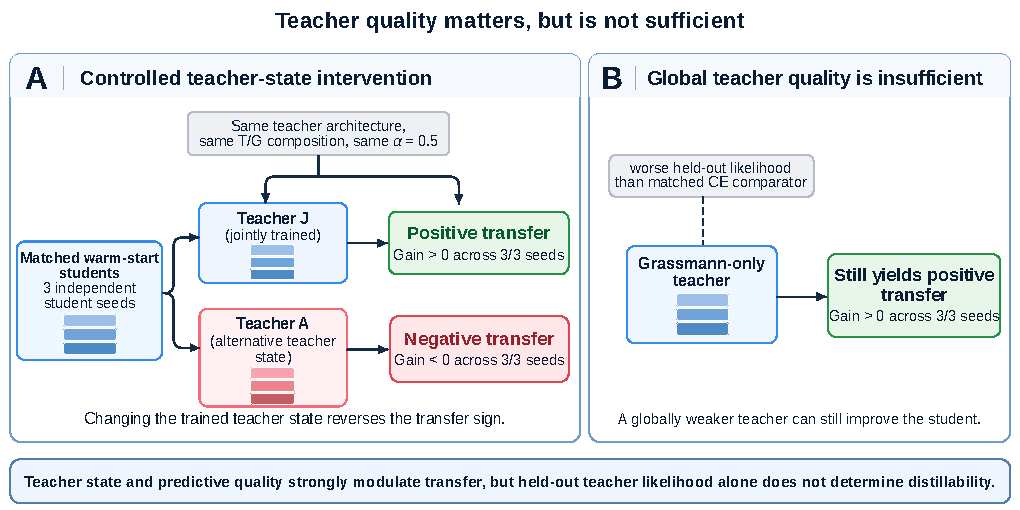
\includegraphics[width=\textwidth]{figures/fig3_teacher_quality.pdf}
\caption{WikiText-2 的状态与似然对照。在固定组成下，改变已训练的教师模型状态会反转迁移符号；似然差于 CE 的监督源仍能产生正迁移。这两项结果均不证明标量似然的因果作用或几何结构带来的 KD 优势。}
\label{fig:teacher_quality}
\end{figure}
